\subsection{IllustrisTNG}
IllustrisTNG \footnote{https://www.tng-project.org/} is the follow-up project after the success of the Illustris simulations \parencite{Springel2017, Pillepich2017,Naiman2018, Nelson2017, Marinacci2018}. It is a huge project, built upon a magneto-hydrodynamical cosmological simulation code with added physical processes on a subgrid level \parencite{Weinberger2016}. Adding physical processes like gas radiation, star formation, stellar feedback through supernova explosions, supermassive black hole accretion and magnetic fields is essential to model galaxy formation and evolution and allows for a much better comparison to reality compared to dark matter-only simulations. The data output from the simulations is extensive, and is not meant to be analyzed all in one go, but rather through a series of analyzes, each targeting a specific scientific question. 

Hydrodynamical cosmological simulations are used to predict the movements and interactions between different types of particles in a cosmological box, and follow these through time steps as the simulation progresses. In the end, the simulation gives information about the final particle positions and properties. The simulation does not know about halos, so the raw data must be processed to extract information about seperate halos and galaxies. To identify which particles belong together as one halo, their closeness has to be examined, as well as their velocities to see if their kinetic energy is enough to make them gravitationally unbound.

\texttt{SUBFIND} is an algorithm developed by (...Springel et al 2001) for identifying halos and subhalos. It first defines parent halos with a Friends-Of-Friends algorithm, which determines halos by the proximity of the particles only. It then looks at the halo's density fields and separates out subhalos. Finally physically unbound particles (those with positive total energy) are removed. Subhalos identified to reside inside a larger subhalo are counted as a seperate subhalo, and thus its particles are not part of the parent subhalo. The relative mass of a parent subhalo and any subhalos contained within it is usually such that the impact of removing the latter is minimal with respect to any properties of the former.


\subsubsection{The simulations}
The IllustrisTNG project includes 18 different simulations with varying resolutions, spatial size, and included physics. There are three main simulations, TNG300, TNG100, and TNG50, that differ in volume and resolution. The details of these are summed up in Table \ref{TNG}. Each of the main simulations has been run at three different resolution levels, which makes it possible to study how the outcome is affected by changing only the resolution in a given simulation. TNG100 has a physical box volume of $110.7^3 \, $Mpc$^3$, and a baryonic particle resolution of $1.4 \times 10^6 M_{\odot}$, while the TNG300 simulation has a volume of $302.6^3 \, $Mpc$^3$ and a baryonic particle resolution of $1.1 \times 10^7 M_{\odot}$. The newly released third simulation, TNG50, has a smaller volume of $51.7^3 \, $Mpc$^3$, but with a much higher baryonic particle resolution of $8.5 \times 10^4 M_{\odot}$. 

In this project, a large statistical sample of galaxies was needed, as well as a resolved structure of the inner part of the galaxies to calculate the different properties, so the TNG100 simulation was the best choice with respect to size and resolution. The TNG100-1 simulation data, which is the highest available resolution for TNG100, has been used throughout the project and will from now on be referred to as TNG only. A visual representation of parts of the simulations can be seen in Figure \ref{tng_illustration}. For its cosmology parameters TNG uses the results from the Planck Collaboration, which are given by $\Omega_{\Lambda,0} = 0.6911$, $\Omega_{m,0}=0.3089$, $\Omega_{b,0}=0.0486$, $\sigma_8=0.8159$, $n_s=0.9667$ and $h = 0.6774$ \parencite{Planck2016}.

\begin{figure}
    \centering
    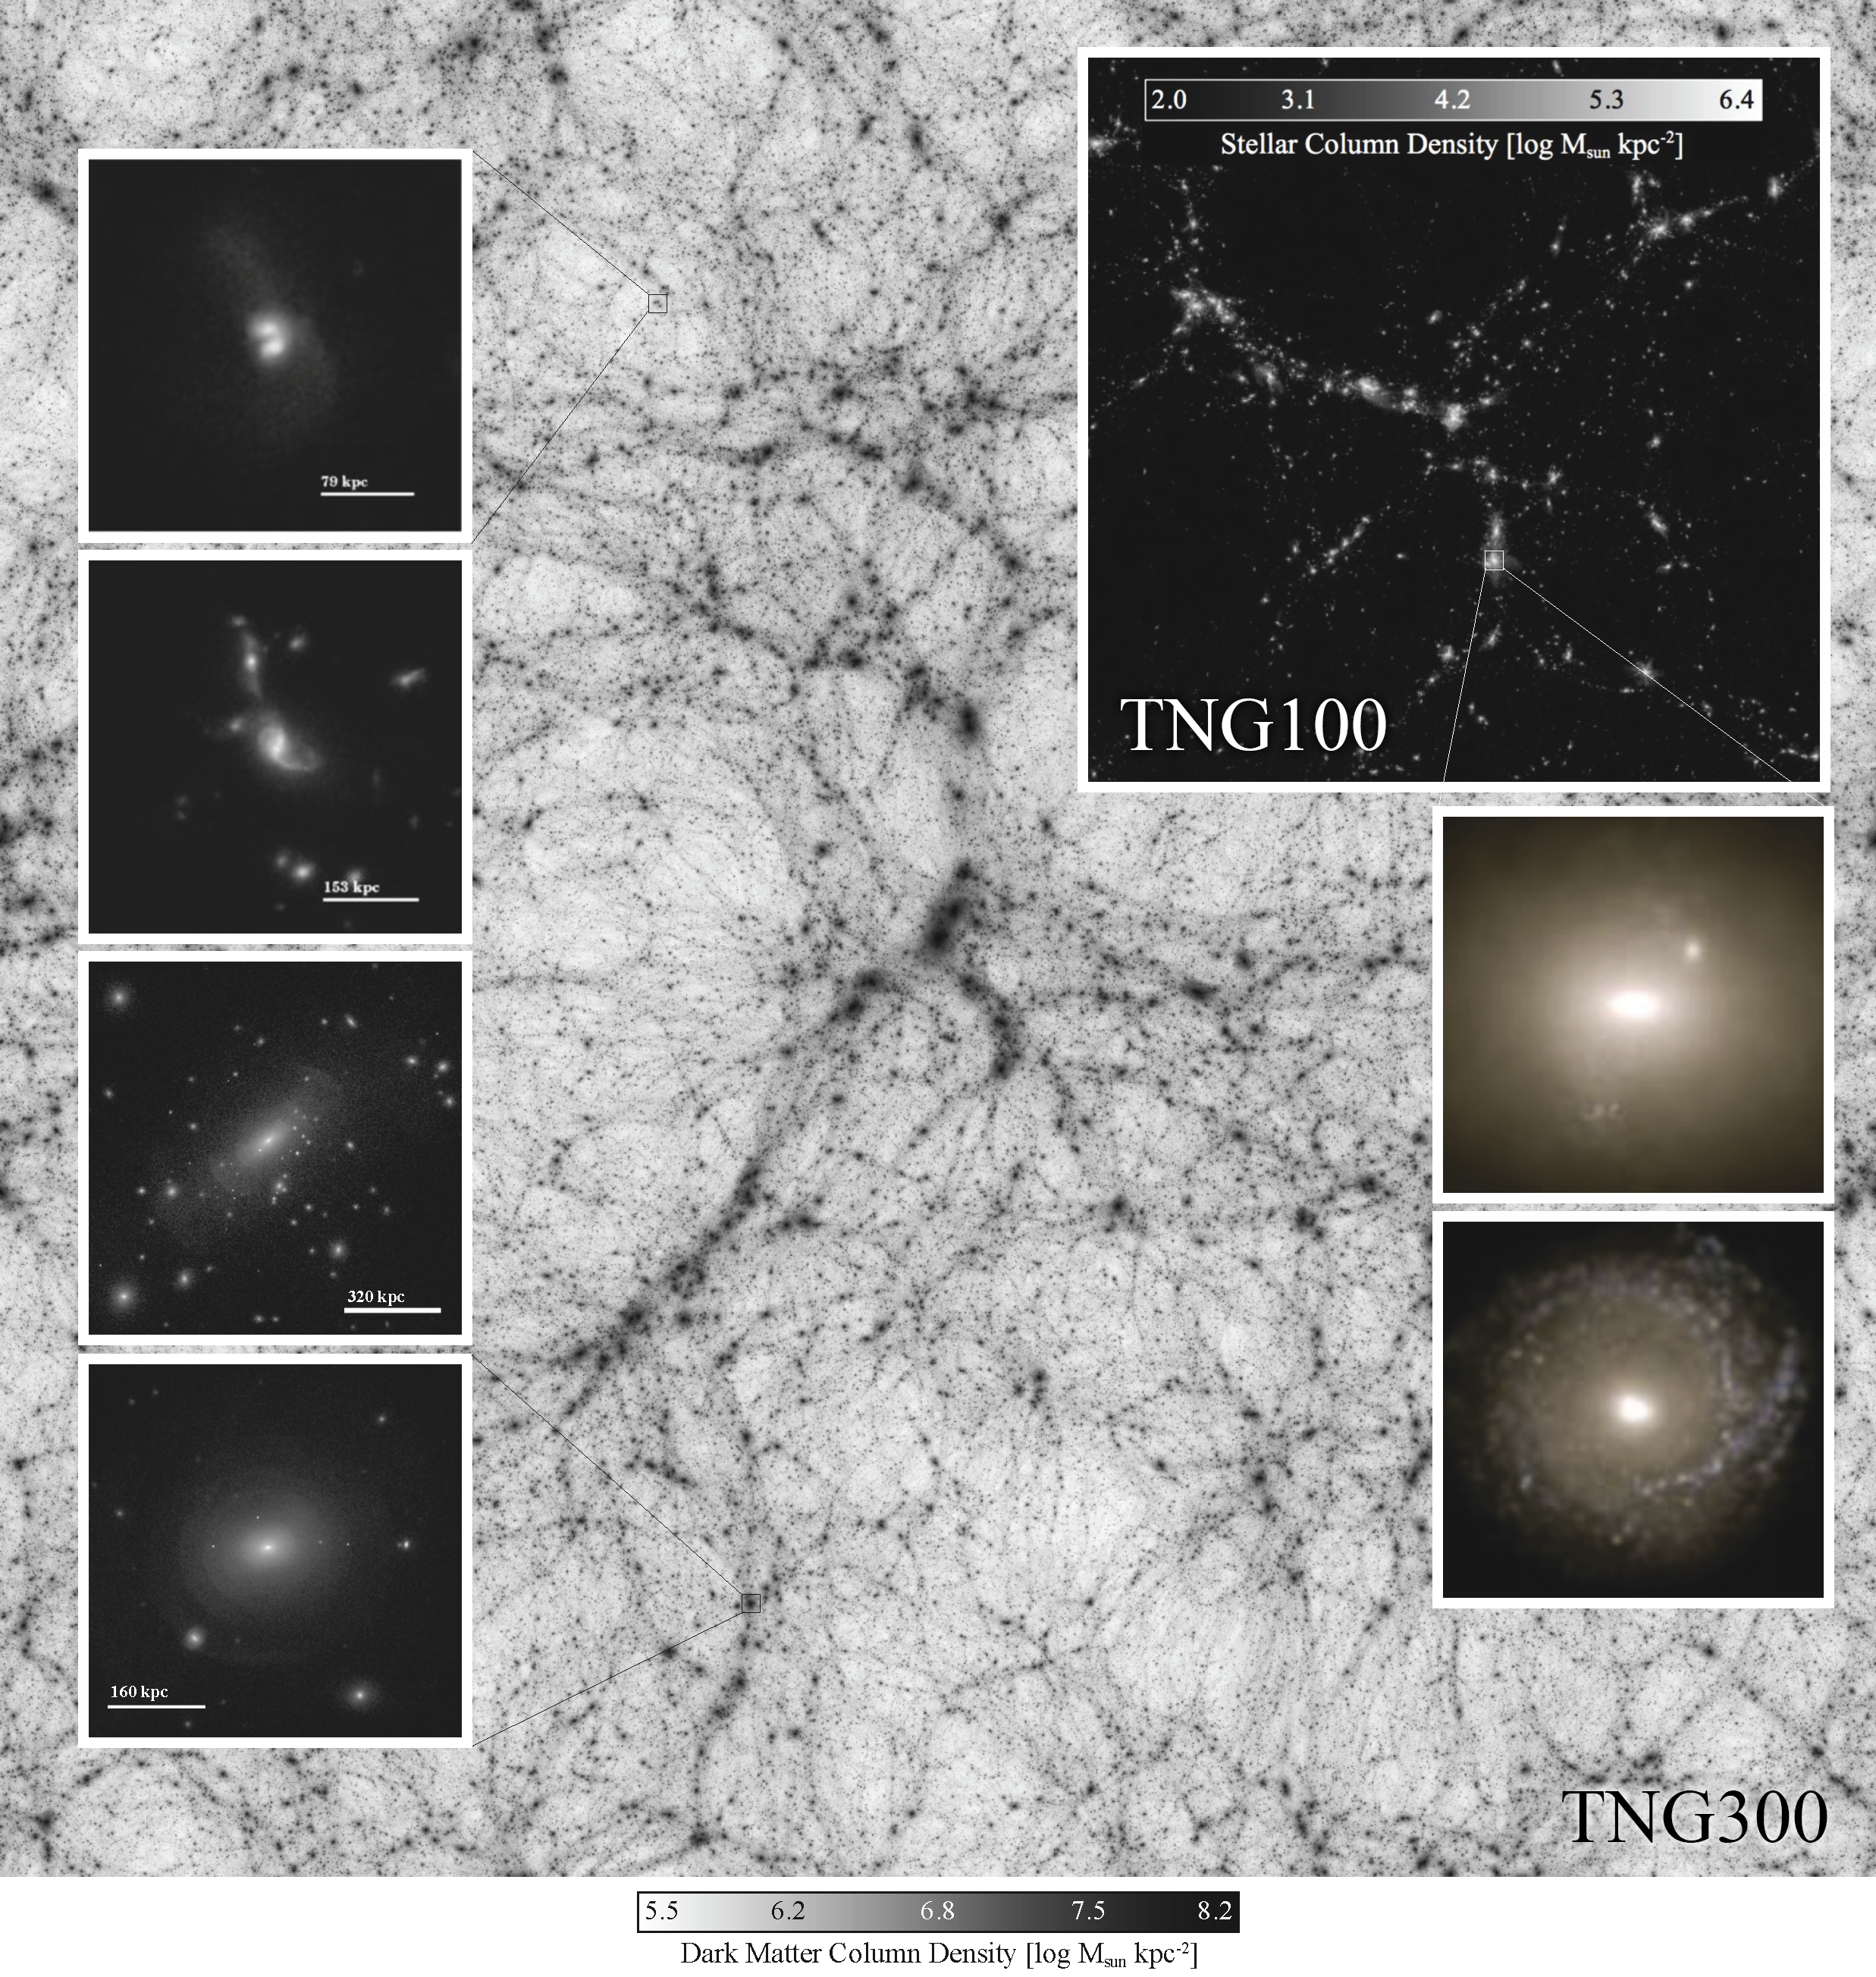
\includegraphics[width=0.9\textwidth]{images/TNG.png}
    \caption{A composite image that illustrates the two simulations TNG100 and TNG300. In the background is the dark matter distribution for the whole TNG300 volume. In the upper right is the stellar mass distribution across the entire TNG100 volume. The panels on the left show galaxy-galaxy interactions, while the panels on the right show the stellar light projections of two $z=0$ galaxies. Credit: TNG Collaboration}.
    \label{tng_illustration}
\end{figure}

\begin{table}
\begin{center}
\caption{The simulation details for the three main TNG simulations. $N_{DM}$ is the amount of dark matter particles. $m_{DM}$ and $m_{baryon}$ is the mass of the dark matter and baryonic particles, respectively.}
 \label{TNG}
\begin{tabular}{ l| c c c c c } 
 \hline
 \hline
   &  Volume [$Mpc^3$] & $N_{DM}$ & $m_{DM}$ [$M_{\odot}$] & $m_{baryon}$ [$M_{\odot}$] \\
 \hline
 TNG50 & $51.7^3$ & $2163^3$ & $4.5 \times 10^5 $ & $8.5 \times 10^4 $ \\ 
 TNG100 & $110.7^3$ & $1820^3$ & $7.5 \times 10^6 $ & $1.4 \times 10^6 $  \\ 
 TNG300 & $302.6^3$ & $2500^3$ & $5.9 \times 10^7 $ & $1.1 \times 10^7 $  \\ 
 \hline 
 \end{tabular}
\end{center}
\end{table}

\subsubsection{Data products}
All the Illustris-TNG data is publically available online at the TNG webpage\footnote{https://www.tng-project.org/data/}. The data products that are available for each simulation are snapshots, group catalogs, and merger trees as well as some supplementary data sets. There are five different particle types in the simulations, and each has its properties stored as particle fields. These fields include information like position, kinematic data, and chemical composition. For each different run of the simulation, 100 snapshots are created, which are taken at specific redshifts. They include all the particles in the whole volume of the simulation, with 20 of them including all the fields for each particle as well.

The group catalogs provide a convenient way to quickly access already calculated properties of the different halos and subhalos instead of dealing with all the particles in a snapshot. This saves a lot of time and effort but gives the user less control over what can be analyzed. There is one group catalog for each snapshot, and this includes two types of objects, Friends-of-Friends (FoF) and SUBFIND. The FoF catalog contains all the halos, and the SUBFIND catalog contains all the subhalos and their associated galaxy (if there is any) for each halo. Each subhalo has a parent halo, and the largest subhalo in each halo is the central subhalo. The merger trees data products contain the merger history of each subhalo.

This project makes use of the group catalogs and particles for the $z = 0$ snapshot.

\subsubsection{Sample reduction}

The TNG documentation recommends filtering out all subhalos that are flagged with the $SubhaloFlag$ field, and so these were cut from the data. They are most probably subhalos of non-cosmological origin, and so should not be considered real galaxies.

For this project, only the central galaxies in each halo are selected. The FoF catalog contains the index for the largest subhalo in each halo, so combining this information with the SUBFIND catalog allows one to create a subset of the data that contains only the central galaxies.

Only galaxies with stellar mass greater than $10^{9.5} M_{\odot}$ are used, which corresponds to about 4500 stellar particles.

\subsection{Observational data}
When possible, it is good practice to use the same observational data for comparisons with the simulation data. Trying to accomplish this, in the the SAMI Galaxy Survey \parencite{Bryant2015} has been used throughout this work. For the SHM relation however, it was not possible to use the SAMI data set, so other works have been chosen to use for that comparison. All the data sets and best fits used in comparing the results from TNG to observations are described in this section.

\subsubsection{SAMI Galaxy Survey}
The Sydney–Australian Astronomical Observatory Multi-Object Integral Field Spectrograph (SAMI) is mounted on the Anglo-Saxan telescope in Australia. The SAMI Galaxy Survey \footnote{https://sami-survey.org/} is a spectroscopic survey of a large sample of galaxies in the nearby Universe ($z < 0.113$). The survey was started in 2013, and ended in 2018. There have been two major data releases, with the newest being Data Release Two (DR2) \parencite{Scott2018}. DR2 includes data for 1559 galaxies, which is about 50 \% of the full galaxy survey. The data products available are IFS data cubes and 2D maps, as well as catalogue data. As the same galaxies have been cataloged in several other studies, data products from those studies are added to SAMI data. Analysing data cubes and 2D maps falls outside the scope of this work, so catalogue data is used where possible. 

\subsubsection{Other data sets}
For the SHM relation, best fit models from two different abundance method papers were used in the comparison to TNG.

The first one found a fit to the data by using a power law for the high mass end, and a subpower law for the low mass end \parencite{Behroozi2013}.

\begin{equation} \label{eq_behroozi}
    \log(M_*(M_{halo})) = \log(\epsilon M_1) + f(\log(M_{halo}/M_1)) -f(0),
\end{equation}
\begin{equation*}
    f(x) = -\log(10^{\alpha x}+1)+\delta \frac{(\log(1+\exp(x)))^\gamma}{1 +\exp(10^{-x})}.
\end{equation*}

Here $M_1$ is a characteristic halo mass, $\delta$ is the strength of the subpower law, $\alpha$ is the power law slope for $M_{halo} << M_1$ and $\gamma$ is the power law index for $M_{halo} >> M_1$. The best fit values for the parameters are $M_1 = 11.514\pm(0.053, 0.009)$, $\delta = 3.508 \pm (0.087, -0.369)$, $\alpha = -1.412 \pm (0.020, -0.105)$, $\epsilon = -1.777 \pm (0.133, 0.146)$ and $\gamma = 0.316 \pm (0.076, -0.012)$.

The second one employed the same function for the fit as \textcite{Behroozi2013}, but with different data. The best fit parameters were found to be $M_1 = 11.632\pm(0.008, 0.009)$, $\delta = 3.797 \pm (0.026, 0.021)$, $\alpha = -2.352 \pm (0.026, -0.021)$, $\epsilon = -1.785 \pm (0.010, 0.008)$  and $\gamma = 0.600 \pm (0.10, 0.013)$ \parencite{Zanisi2019}.


\subsection{Calculating properties}

\subsubsection{Cosmologies and h-dependence} \label{cosmologies}
When making measurements of galaxy properties, some assumptions about the underlying cosmology of the Universe must be made. One of these assumptions is the value of the Hubble constant $H_0$, more commonly represented by $h$, where $H_0 = 100\,h\,$ km/s/Mpc. In addition to several other cosmological parameters, this constant is used when running a cosmological simulation. Astrophysical properties, both numerical and observational, are presented in publications with an h-dependence (leaving the user to specify the cosmology) or without an h-dependence (by assuming a value for h).

For IllustrisTNG, $h=0.6774$ and the explicit $h$-dependence of each property value is stated clearly in the documentation. For the SAMI data catalogue, no $h$-dependence is explicitly stated in the documentation or data release papers, but the Hubble constant used is given as $h = 0.7$.

Best practice dictates that to compare works with different assumed Hubble constants, the $h$ used in those specific works should be replaced with the most recent value for $h$ \parencite{Croton2013}. The values for galaxy properties will then be comparable. In Table \ref{h_dependence} the h-dependency of the galaxy properties of TNG as well as the common h-dependencies for observational data is shown along with their corresponding units. In this work, all data results are converted to the TNG cosmology, which uses the newest values for the cosmological parameters.

\begin{table}
\begin{center}
\caption{The $h$-dependence and units for the galaxy properties used in this work. For TNG, the dependency is given in the data documentation. The dependencies for SAMI are the standard dependencies for observational data, as found in Table 2 in \textcite{Croton2013}.}
\label{h_dependence}
\begin{tabular}{ l| c c }
 \hline
 \hline
   & TNG & SAMI \\
 \hline
 Stellar mass & $M_{\odot}h^{-1}$ & $M_{\odot}h^{-2}$ \\ 
 Halo mass & $M_{\odot}h^{-1}$ & - \\
 Size & kpc$\,h^{-1}$ & kpc$\,h^{-1}$ \\
 Luminosity & mag & mag $+5\log(h)$ \\
 Velocity & km/s & km/s  \\ 

 \hline 
\end{tabular}
\end{center}
\end{table}

\subsubsection{Galaxy sizes} \label{galaxy_size}
When observing galaxies with telescopes, there is always the problem of contamination of the measurements by surrounding sources as well as background radiation. As such, when the images are processed, aperture sizes have to be chosen with care for each identified galaxy. A larger aperture will be sure to contain most of the light from the galaxy but might overshoot by including surrounding light as well. However, choosing a too small aperture will result in lost data, and as such a smaller apparent galaxy. Usually a circular or elliptical aperture with a calculated radius to balance these two issues is chosen.

In simulations, we are not limited by hardware, attenuation, and background light. A cut-off point still needs to be determined. \texttt{SUBFIND} does this for the dark matter part of the simulation, separating out subhalos from larger halos. The galaxy properties of that subhalo are then calculated using all the stellar and gas particles in the subhalo and saved in the group catalog. 

When comparing simulation data to observational data, there are many ways to emulate the finite size of observed galaxies. Calculating luminosities and selecting a cut-off point at the faint end, using a spherical volume with a radius that is a multiple of their particular effective radius, or a fraction of the virial radius of the parent subhalo are some of the most commonly employed methods. In \textcite{Pillepich2017} users of TNG data are urged to consider their choice of aperture size with caution and emphasise that the definitions must always be stated clearly. They adovcate the use of a simple galaxy radius of some fixed aperture in physical kiloparsecs.

\subsubsection{Magnitude and colors}

The absolute magnitude ($\mathcal{M}$) is a measure of the total luminosity ($L$) of the galaxy such that $\mathcal{M} = -2.5 \log(L/L_\odot) + \mathcal{M}_\odot$, where $L_\odot$ is the solar luminosity and $\mathcal{M}_\odot$ is the solar magnitude.

For the \texttt{SUBFIND} group catalog, the \texttt{SubhaloStellarPhotometrics} field gives the magnitudes based on the summed up luminosities of all the stellar particles in the Subhalo. The particle luminosities are determined by summing the luminosities within $R_{gal}$. Eight bands are available, but here only the g- and i-band are used. 

The g-i colors for the particles are calculated by simply subtracting the i-band magnitude from the g-band magnitude.

In SAMI, g-i color values are adopted from the GAMA Sérsic catalogue \parencite{Driver2011}.

\subsubsection{Masses}

Stellar mass estimates depend on the stellar initial mass function (IMF), which describe the spectral evolution of a population of stars, and as such the relationship between luminosity and mass in a given spectral band. SAMI and TNG both adopt a \textcite{Chabrier2003} IMF.

In \texttt{SUBFIND}, masses for each particle type are calculated by summing up all the masses of that particle type belonging to the subhalo. Values for the mass within the stellar half-mass radius, two times the stellar half-mass radius and the radius at which the maximum rotational velocity is found are also available.

//Write more about the mass within 30 kpc etc. The high-mass end results from Pillepich. 

For SAMI DR2, the stellar mass values are taken from the GAMA Sérsic catalogue \parencite{Driver2011}. They calculate the stellar masses by using the i-band magnitude and g-i color of each galaxy through the formula $\log(M_*/M_\odot) = 1.15 + 0.70(g-i) -0.4\mathcal{M}_i$, where $\mathcal{M}_i$ is the rest-frame i-band absolute magnitude \parencite{Taylor2011}.

\subsubsection{Size}

In observational data, galaxy sizes are always projected sizes, as they are derived from 2D images. A common measure of the size of a galaxy is the effective radius ($R_e$), which is the radius within which half the light of the galaxy is contained. This quantity depends on the analysis and quality of the 2D profiles, and may not be able to include all the light in a galaxy in the way that we can ensure for computer simulated data. The radius also depends on which optical filter the measurements are made in, as different filters will be receptive to light from different parts of the galaxy. To be consistent with the simulation data, the 2D radius from the observations are projected by using the relation $r_{1/2} = \frac{4}{3}R_{e}$, where $r_{1/2}$ is the 3D deprojected half-light radius and $R_e$ is the 2D projected half-light radius, which generally holds for a range of surface brightness profiles observed in stellar systems \parencite{Wolf2010}.

For TNG data, the \texttt{SubhaloHalfmassRadStellar} field has been used. The half-mass radius is the radius of a spherical volume within which half the stellar mass is found. It is the 3D half-mass radius ($r_hm$), as it is not a projected quantity. This value is generally higher than the 2D half-light radius ($R_{hl}$) for a given mass up to $M_{*} < 10^{10.5}$, as seen in \textcite{Genel2017}. 

The half-mass radii of the galaxies calculated using the particles are derived using the same method, but using only the total stellar mass calculated within $R_{gal}$.

The SAMI catalog data takes the values for the effective radius from the GAMA Sérsic catalogue \parencite{Driver2011}. The effective radius is defined as the semi-major axis half-light radius, measured in the r-band. The values are given in units of arcsec which were then converted to a physical radius in kpc. //Write about MGE and the other// 

Then these semi-major axis radii are converted to circular radii using the formula

\begin{equation}
   r_{circ} = r_{sm}\sqrt{(1-\epsilon)},
\end{equation}

where $r_{circ}$ is the circular radius, $r_{sm}$ is the semi-major axis effective radius and $\epsilon$ is the eccentricity.


\subsubsection{Velocities}

Galaxy velocities are usually given by the velocity dispersion and rotational velocity for early and late-type galaxies, respectively. This is because of the difference in the shape of the two galaxy types. It makes more sense to talk about velocity dispersion in a spheroidal pressure-dominated system and rotational velocity in a rotating disk.

In \texttt{SUBFIND}, the field \texttt{SubhaloVMax} gives the maximum value for the spherically averaged rotation curve of a given galaxy. As the rotational curves are nearly flat for large enough radii, it should not be very important at which specific radius the observational rotational velocity is measured, as long as it is in the flat part of the curve. For observational data, a common practice is to look at the rotational velocities of stars in the outer part of the galaxy. 

Rotational velocities were not available as SAMI catalogue data, but an extensive analysis of the 2D velocity maps in DR2 is found in \textcite{Bloom2017}. They defined the rotational velocity as the velocity at $2.2\, r_e$, which should be in the flat regime of the velocity curve, and coincide well with the maximum velocity. Their best fit for the TFR was used in our comparison, 
\begin{equation}
	\log(V_{rot}) = 0.31 \pm 0.0092 \times \log(M_*)-0.93 \pm 0.1.
\end{equation}

//To compare with \texttt{SUBFIND}'s \texttt{SubhaloVMax}, the rotational velocity at a radius of $2.2 \times R_e$ was calculated for all galaxies.



If the velocity dispersion tends to fall off at larger radii, and the galaxy has an ellipsoid shape, the angle at which the galaxy is viewed will affect the observed velocity dispersion. To compensate for this when comparing simulations to observations, velocity dispersions in simulations may be calculated in three different projections of the galaxy and averaged over these. 

\begin{equation} \label{sigma1}
    \sigma^{2} = \frac{1}{3}(\sigma_x^2 + \sigma_y^2 + \sigma_z^2)
\end{equation}



In \texttt{SUBFIND}, the velocity dispersion is simply calculated as the velocity dispersion of all the particles over the entire subhalo.

In SAMI catalog data, the given velocity dispersion is averaged within an aperture with radius equal to the effective radius of each galaxy.

With the particles the velocity dispersion was calculated within the projected half-mass radius in three orthogonal projections.


\subsection{Galaxy morphology classifications}

Starting off with the same subset of 5877 galaxies for both the \texttt{SUBFIND} group catalogue and the particles, we get different results for which galaxies are early- and late-type galaxies, based on the volume in which the gas mass is measured. Table \ref{gas_frac} show the number of early and late type galaxies for different volumes.

//UPDATE this with new numbers

\begin{table}
\begin{center}
\caption{Gas fraction.}
 \label{gas_frac}
\begin{tabular}{ l| c c c c c } 
 \hline
 \hline
   &\multicolumn{2}{c}{\texttt{SUBFIND}}&\multicolumn{2}{c}{Particles} \\
   &  Early-type & Late-type & Early-type & Late-type \\
 \hline
 Half-mass radius & 2438 & 3439 & 2479 & 3398 \\ 
 2 $\times$ half-mass radius & 1818 & 4059 & 1920 & 3957 \\ 
 15\% R$_{200}$ & - & - & 799 & 5078 \\ 
 R$_{subhalo}$ & 63 & 5814 & - & - \\ 
 \hline 
 \end{tabular}
\end{center}
\end{table}

The selection process using the sSFR with $ -1.44 < \log (sSFR[Gyr^{-1}]) $ being late type and $\log (sSFR[Gyr^{-1}]) < -1.94$ being early type gives very similar results whether \texttt{SUBFIND} or particles are used. For \texttt{SUBFIND} we get 1350 early-types, 4129 late-types and 398 intermediate types, while for the particles we find 1365 early-types and 4129 late-type galaxies with 383 intermediate types.

By using the simple cut at $\kappa_{rot} = 0.6$ the 5877 galaxies are then separated into 4359 early type galaxies and 1518 late types. This is a completely different result from the two methods above, where there was a majority of late-type galaxies. In real life we know that smaller late-type galaxies dominate, so using only the rotational energy does not yield the expected ratio. However, combining this result with one of the two above should result in a subset of galaxies which exhibit both the right amount of cold gas and the star formation that goes with it, as well as the right kinematic structure.

In the rest of this paper, early-type galaxies are those which, calculated using the particles, have a sSFR of $\log (sSFR[Gyr^{-1}]) < -1.94$ as well as $\kappa_{rot} < 0.6$. Late-types have a sSFR of $ -1.44 < \log (sSFR[Gyr^{-1}]) $ as well as $\kappa_{rot} > 0.6$. This results in 1228 early-type galaxies, 1300 late-types and 3349 intermediate-type galaxies. For the \texttt{SUBFIND} sample, the same galaxies in each group are chosen by matching the subhalo-id from the previously mentioned selection. //Insert figure of galaxies.